\documentclass{article}

\usepackage{arxiv}

\usepackage[utf8]{inputenc} % allow utf-8 input
\usepackage[T1]{fontenc}    % use 8-bit T1 fonts
\usepackage{hyperref}       % hyperlinks
\usepackage{url}            % simple URL typesetting
\usepackage{booktabs}       % professional-quality tables
\usepackage[english]{babel}
\usepackage{amsthm}
\usepackage{amsfonts}       % blackboard math symbols
\usepackage{nicefrac}       % compact symbols for 1/2, etc.
\usepackage{microtype}      % microtypography

\usepackage{graphicx}
\usepackage{amsmath}

\newtheorem{definition}{Definition}
\newtheorem{lemma}{Lemma}
\newtheorem{proposition}{Proposition}
\newtheorem{program}{Program}
\newtheorem{convention}{Convention}
\newtheorem{theorem}{Theorem}

\usepackage{stmaryrd}
\usepackage{mathtools}

\usepackage{tikz}

\title{Suan: towards a geometry of computation}

%\date{September 9, 1985}	% Here you can change the date presented in the paper title
%\date{} 					% Or removing it

\author{
  Mingli~Yuan \\
  AI Lab \\
  ColorfulClouds Tech.\\
  Beijing, 100083 \\
  \texttt{mingli.yuan@caiyunapp.com} \\
  %% examples of more authors
  %% \AND
  %% Coauthor \\
  %% Affiliation \\
  %% Address \\
  %% \texttt{email} \\
  %% \And
  %% Coauthor \\
  %% Affiliation \\
  %% Address \\
  %% \texttt{email} \\
  %% \And
  %% Coauthor \\
  %% Affiliation \\
  %% Address \\
  %% \texttt{email} \\
}

% Uncomment to remove the date
%\date{}

% Uncomment to override  the `A preprint' in the header
%\renewcommand{\headeright}{Technical Report}
%\renewcommand{\undertitle}{Technical Report}

\begin{document}
\maketitle

\begin{abstract}
    Begin from an embedding of addition-multiplication computation into hyperbolic surface, we define a local polar
    coordinate on hyperbolic surface and then derive a flow equation, after studying several examples, we proof the
    consistency among the discrete constructions, infinitesimal calculation and the hyperbolic geometrical structures, and
    these lead us to a new mathematical system $\mathfrak{S}$.
\end{abstract}

\keywords{hyperbolic surface \and addition-multiplication tree \and infinitesimal calculation \and Suan system \and surreal number \and geometry of computation}

\setcounter{tocdepth}{2}
\tableofcontents

\section{Arithmetical expressions}\label{sec:expressions}

\begin{lemma}
\label{lemma:arithmeticalalgebra}
All arithmetical expressions $A$ over real number $R$ is an algebra $\mathcal{A} = (A, R, \cdot)$.
\end{lemma}

\begin{proof}
It is easy to verify the three axioms should be hold by an algebra:
for any arithmetical expressions $x$, $y$, $z$ and real number $a$, $b$, we have
\begin{itemize}
    \item right distributivity: $(x + y) \cdot z = x \cdot z + y \cdot z$
    \item left distributivity: $z \cdot (x + y) = z \cdot x + z \cdot y$
    \item compatibility with scalars: $(ax) \cdot (by) = (ab) (x \cdot y)$
\end{itemize}
\qedhere
\end{proof}

It should be noticed that the equality here is equality from R which applying on the calculation result of each expressions.
We just omitted the technical details of the inductions over the recursive definition of $A$.

Euler's number $e$ is irrational and transcendental, the first 50 decimals of e is
$$
e = 2.71828182845904523536028747135266249775724709369995...
$$

Now we consider the arithmetical expression set $A_n$ which is freely generated from
\begin{itemize}
    \item initial operand: $0$
    \item operator $\oplus_n: x \mapsto x + 2^{-n}$
    \item operator: $\ominus_n: x \mapsto x - 2^{-n}$
    \item operator: $\otimes_n: x \mapsto x \cdot e^{2^{-n}}$
    \item operator: $\oslash_n: x \mapsto x / e^{2^{-n}}$
\end{itemize}
where e is the Euler's number.

With $A_n$ defined as above, we have a chain of inclusion
\begin{lemma}
\label{lemma:chainofinclusion}
We have
$$ A_0 \subset A_1 \subset A_2 \subset \ldots \subset A_n \subset \ldots $$
hold for all $n$.
\end{lemma}

\subsection{Syntactical conclusions from the generating}\label{sec:generating}

In this section, we discus the conclusions that is drawn only from the syntactical side of the definition of $A_n$ and
do not borrow any semantic properties from the algebra of the expressions $\mathcal{A}$.

The inverse notion can be introduced
\begin{itemize}
    \item $\oplus_n^{-1} = \ominus_n$
    \item $\ominus_n^{-1} = \oplus_n$
    \item $\otimes_n^{-1} = \oslash_n$
    \item $\oslash_n^{-1} = \otimes_n$
\end{itemize}

Suppose we have a operand $\alpha \in A_n $ and a series of operators $a_1, a_2, ... a_{n-1}, a_n$,
we introduce the path notion:
$$\alpha a_1 a_2 ... a_{n-1} a_n = a_n( a_{n-1}( ... a_2( a_1(\alpha) ) ... ) )$$

Then we have the calculation rule of inverse.

\begin{lemma}
\label{lemma:inverserule}
If we have
$$\beta = \alpha a_1 a_2 ... a_{n-1} a_n$$
then
$$\alpha = \beta a_n^{-1} a_{n-1}^{-1} ... a_2^{-1} a_1^{-1}$$
\end{lemma}

\begin{proof}
Notice that $\oplus_n, \ominus_n, \otimes_n, \oslash_n$ are all bijections, we know that $\alpha a_1 a_2 ... a_{n-1} a_n$ is a composition of functions

$$\beta = a_n( a_{n-1}( ... a_2( a_1(\alpha) ) ... ) )$$

Considering the inverse of a composition, we have

$$\alpha = a_1^{-1}( a_2^{-1}( ... a_{n-1}^{-1}( a_n^{-1}(\beta) ) ... ) )$$

Or under the path notion

$$\alpha = \beta a_n^{-1} a_{n-1}^{-1} ... a_2^{-1} a_1^{-1}$$

\qedhere
\end{proof}

After intruduce of a zero operator $\odot$ which is its own inverse:
\begin{itemize}
    \item $\odot: x \mapsto x$
    \item $\odot^{-1} = \odot$
\end{itemize}

Informally We can divide a long calculation into pieces, or composite small pieces of calculations into a longer one,
for example

$$\gamma = 0 a_1 a_2 ... a_{n-1} a_n b_1 b2 ... b_{m-1} b_m$$

can be rewritten as

$$\gamma = 0 ((\odot a_1 a_2 ... a_{n-1} a_n) \circ (\odot b_1 b_2 ... b_{m-1} b_m))$$

And if we treat $\odot$ and $0$ as the same, and we define

$$\alpha = 0 a_1 a_2 ... a_{n-1} a_n$$
$$\beta = 0 b_1 b2 ... b_{m-1} b_m$$

We have

$$\gamma = \alpha \circ \beta$$

where $\alpha$, $\beta$ and $\gamma$ are all well defined in of $A_n$.

It is easy to see the algebraic structure $\mathcal{P}_n = (A_n, \circ)$ is a group, and we call it \emph{path group}.

\begin{figure}[ht]
\centering
\begin{tikzpicture}

\filldraw [black] (0,0) circle (2pt) node[align=center, below] {0};
\filldraw [black] (4,1) circle (2pt) node[align=center, below] {$\alpha$};
\filldraw [black] (2,3) circle (2pt) node[align=center, below] {$\beta$};
\filldraw [black] (5,3) circle (2pt) node[align=center, below] {$\gamma$};
\filldraw [black] (-2,2) circle (2pt) node[align=center, below] {$\psi$};
\filldraw [black] (1,2) circle (2pt) node[align=center, below] {$\phi$};
\filldraw [gray] (3,-0.4) circle (0pt) node[align=center, below] {$x$};
\filldraw [gray] (3,1.8) circle (0pt) node[align=center, below] {$y$};
\filldraw [gray] (4.7,2) circle (0pt) node[align=center, below] {$z$};
\draw [gray] (0,0) to[out=300,in=240] (4,1);
\draw [gray] (4,1) to[out=120,in=300] (2,3);
\draw [gray] (4,1) to[out=60,in=240] (5,3);
\draw [gray] (0,0) to[out=120,in=300] (-2,2);
\draw [gray] (0,0) to[out=60,in=240] (1,2);
\filldraw [gray] (-1,0.8) circle (0pt) node[align=center, below] {$y$};
\filldraw [gray] (0.7,1) circle (0pt) node[align=center, below] {$z$};

\end{tikzpicture}
\caption{Factorization by greatest common divisor}
\end{figure}

\begin{lemma}
\label{lemma:coprimes}
When $\alpha = gcd(\beta, \gamma)$, and $\beta = \alpha \circ \psi$, $\gamma = \alpha \circ \phi$ hold, we have $\psi$ and $\phi$ are coprimes.
\end{lemma}


\subsection{Semantic conclusions from the calculation}\label{sec:calculation}

In this section, we study the conclusions related with the calculation result in $\mathcal{A}$ for each expression of $A_n$.
For example, we can verify path group $\mathcal{P}_n$ is non-abelian by calculating the result at point $0$.

\begin{lemma}
\label{lemma:nonabelian}
The path group $\mathcal{P}_n = (A_n, \circ)$ is non-abelian
\end{lemma}

\begin{proof}
Notice that $0 \oplus_n \otimes_n \neq 0 \otimes_n \oplus_n$
\qedhere
\end{proof}

The result of each calculation is a mapping $Val$ from $A_n$ to real number $R$
$$ Val: A_n \to R $$

But not an arbitrary function from $A_n$ to $R$ can take the role of $Val$ here,
because $Val$ is uniformed under the generating relationship.



We can consider two subgroup $\mathcal{N}_n$ and $\mathcal{Q}_n$ of $\mathcal{P}_n$.

The subgroup $\mathcal{N}_n$ are all expressions freely generated from
\begin{itemize}
    \item initial operand: $0$
    \item operator: $\otimes_n: x \mapsto x \cdot e^{2^{-n}}$
    \item operator: $\oslash_n: x \mapsto x / e^{2^{-n}}$
\end{itemize}

The subgroup $\mathcal{Q}_n$ of $\mathcal{P}_n$ are all expressions freely generated from
\begin{itemize}
    \item initial operand: $0$
    \item operator $\oplus_n: x \mapsto x + 2^{-n}$
    \item operator: $\ominus_n: x \mapsto x - 2^{-n}$
\end{itemize}

\begin{figure}[ht]
\centering
\begin{tikzpicture}

\filldraw [black] (0,0) circle (2pt) node[align=center, below] {0};
\filldraw [black] (0,4) circle (2pt) node[align=center, right] {$\alpha = \beta^{-1} \circ \alpha \circ \beta$};
\filldraw [black] (2,1) circle (2pt) node[align=center, right] {$\beta$};
\filldraw [black] (-2, -1) circle (2pt) node[align=center, left] {$\beta^{-1}$};
\filldraw [black] (-2, 3) circle (2pt) node[align=center, left] {$\beta^{-1} \circ \alpha$};
\filldraw [gray] (-0.4, 2) circle (0pt) node[align=center, below] {$n$};
\filldraw [gray] (-2.4, 1) circle (0pt) node[align=center, below] {$n$};
\filldraw [gray] (1, 0.3) circle (0pt) node[align=center, below] {$x$};
\filldraw [gray] (-1, -0.5) circle (0pt) node[align=center, below] {$x^{-1}$};
\draw [gray] (0,0) to[out=90,in=270] (0,4);
\draw [gray] (0,0) to[out=330,in=180] (2,1);
\draw [gray] (0,0) to[out=150,in=0] (-2,-1);
\draw [gray] (-2,-1) to[out=90,in=270] (-2,3);
\draw [gray] (-2,3) to[out=330,in=180] (0,4);

\end{tikzpicture}
\caption{If $\mathcal{N}_n $ is normal}
\end{figure}

\begin{lemma}
\label{lemma:normalofn}
The subgroup $\mathcal{N}_n $ is a normal subgroup of $\mathcal{P}_n$.
\end{lemma}

\begin{proof}
?
\qedhere
\end{proof}

\begin{figure}[ht]
\centering
\begin{tikzpicture}

\filldraw [black] (0,0) circle (2pt) node[align=center, left] {0};
\filldraw [black] (4,0) circle (2pt) node[align=center, right] {$\alpha = \beta^{-1} \circ \alpha \circ \beta$};
\filldraw [black] (1,2) circle (2pt) node[align=center, below] {$\beta$};
\filldraw [black] (-1,-2) circle (2pt) node[align=center, below] {$\beta^{-1}$};
\filldraw [black] (3,-2) circle (2pt) node[align=center, below] {$\beta^{-1} \circ \alpha$};
\filldraw [gray] (2,-0.4) circle (0pt) node[align=center, below] {$q$};
\filldraw [gray] (1,-2.4) circle (0pt) node[align=center, below] {$q$};
\filldraw [gray] (0.7,1) circle (0pt) node[align=center, below] {$x$};
\filldraw [gray] (-0.1,-1) circle (0pt) node[align=center, below] {$x^{-1}$};
\draw [gray] (0,0) to[out=0,in=180] (4,0);
\draw [gray] (0,0) to[out=90,in=240] (1,2);
\draw [gray] (0,0) to[out=-90,in=60] (-1,-2);
\draw [gray] (-1,-2) to[out=0,in=180] (3,-2);
\draw [gray] (3,-2) to[out=90,in=240] (4,0);

\end{tikzpicture}
\caption{If $\mathcal{Q}_n $ is normal}
\end{figure}

\begin{lemma}
\label{lemma:normalofq}
The subgroup $\mathcal{Q}_n $ is a normal subgroup of $\mathcal{P}_n$.
\end{lemma}

\begin{proof}
?
\qedhere
\end{proof}

A kind of duality of the above two subset are there, duals to measure the regularity and transcendentality.

There should be a transcendental dual of below regular formula
$$ e = \sum_{n = 0}^\infty \frac{1}{n!} = \frac{1}{0!} + \frac{1}{1!} + \frac{1}{2!} + \frac{1}{3!} + \frac{1}{4!} + \cdots $$

I still need time to figure it out, but clues include

$$ e = \sum_{n = 1}^\infty \frac{1}{\Gamma(n)} = \frac{1}{\Gamma(1)} + \frac{1}{\Gamma(2)} + \frac{1}{\Gamma(3)} + \frac{1}{\Gamma(4)} + \frac{1}{\Gamma(5)} + \cdots $$

$$ e = \sum_{k = 1}^\infty \frac{1}{\Gamma(k)} = \sum_{k = 1}^\infty k e^{\gamma k} \prod_{n=1}^\infty \left(1 + \frac{k}{n}\right) e^{-\frac{k}{n}} $$

$$\cdots$$

I need to convert the above into an identity with $1$ in the left side and an infinite product in the right side.

The other candidate is

$$
\lim_{n \to \infty} \frac{(n!)^{1/n}}{n} = \frac{1}{e}
$$

\subsection{Lindemann–Weierstrass theorem}\label{sec:lindemann}

\section{An embedding from generated expressions to hyperbolic surface}\label{sec:embeding}

$A_0$ can be embedded into Hyperbolic plane $H_2$ as a regular tree which is an infinite tree of degree 4.

\begin{figure}[ht]
\centering
\begin{tikzpicture}
    \draw (0, 0) node[inner sep=0] {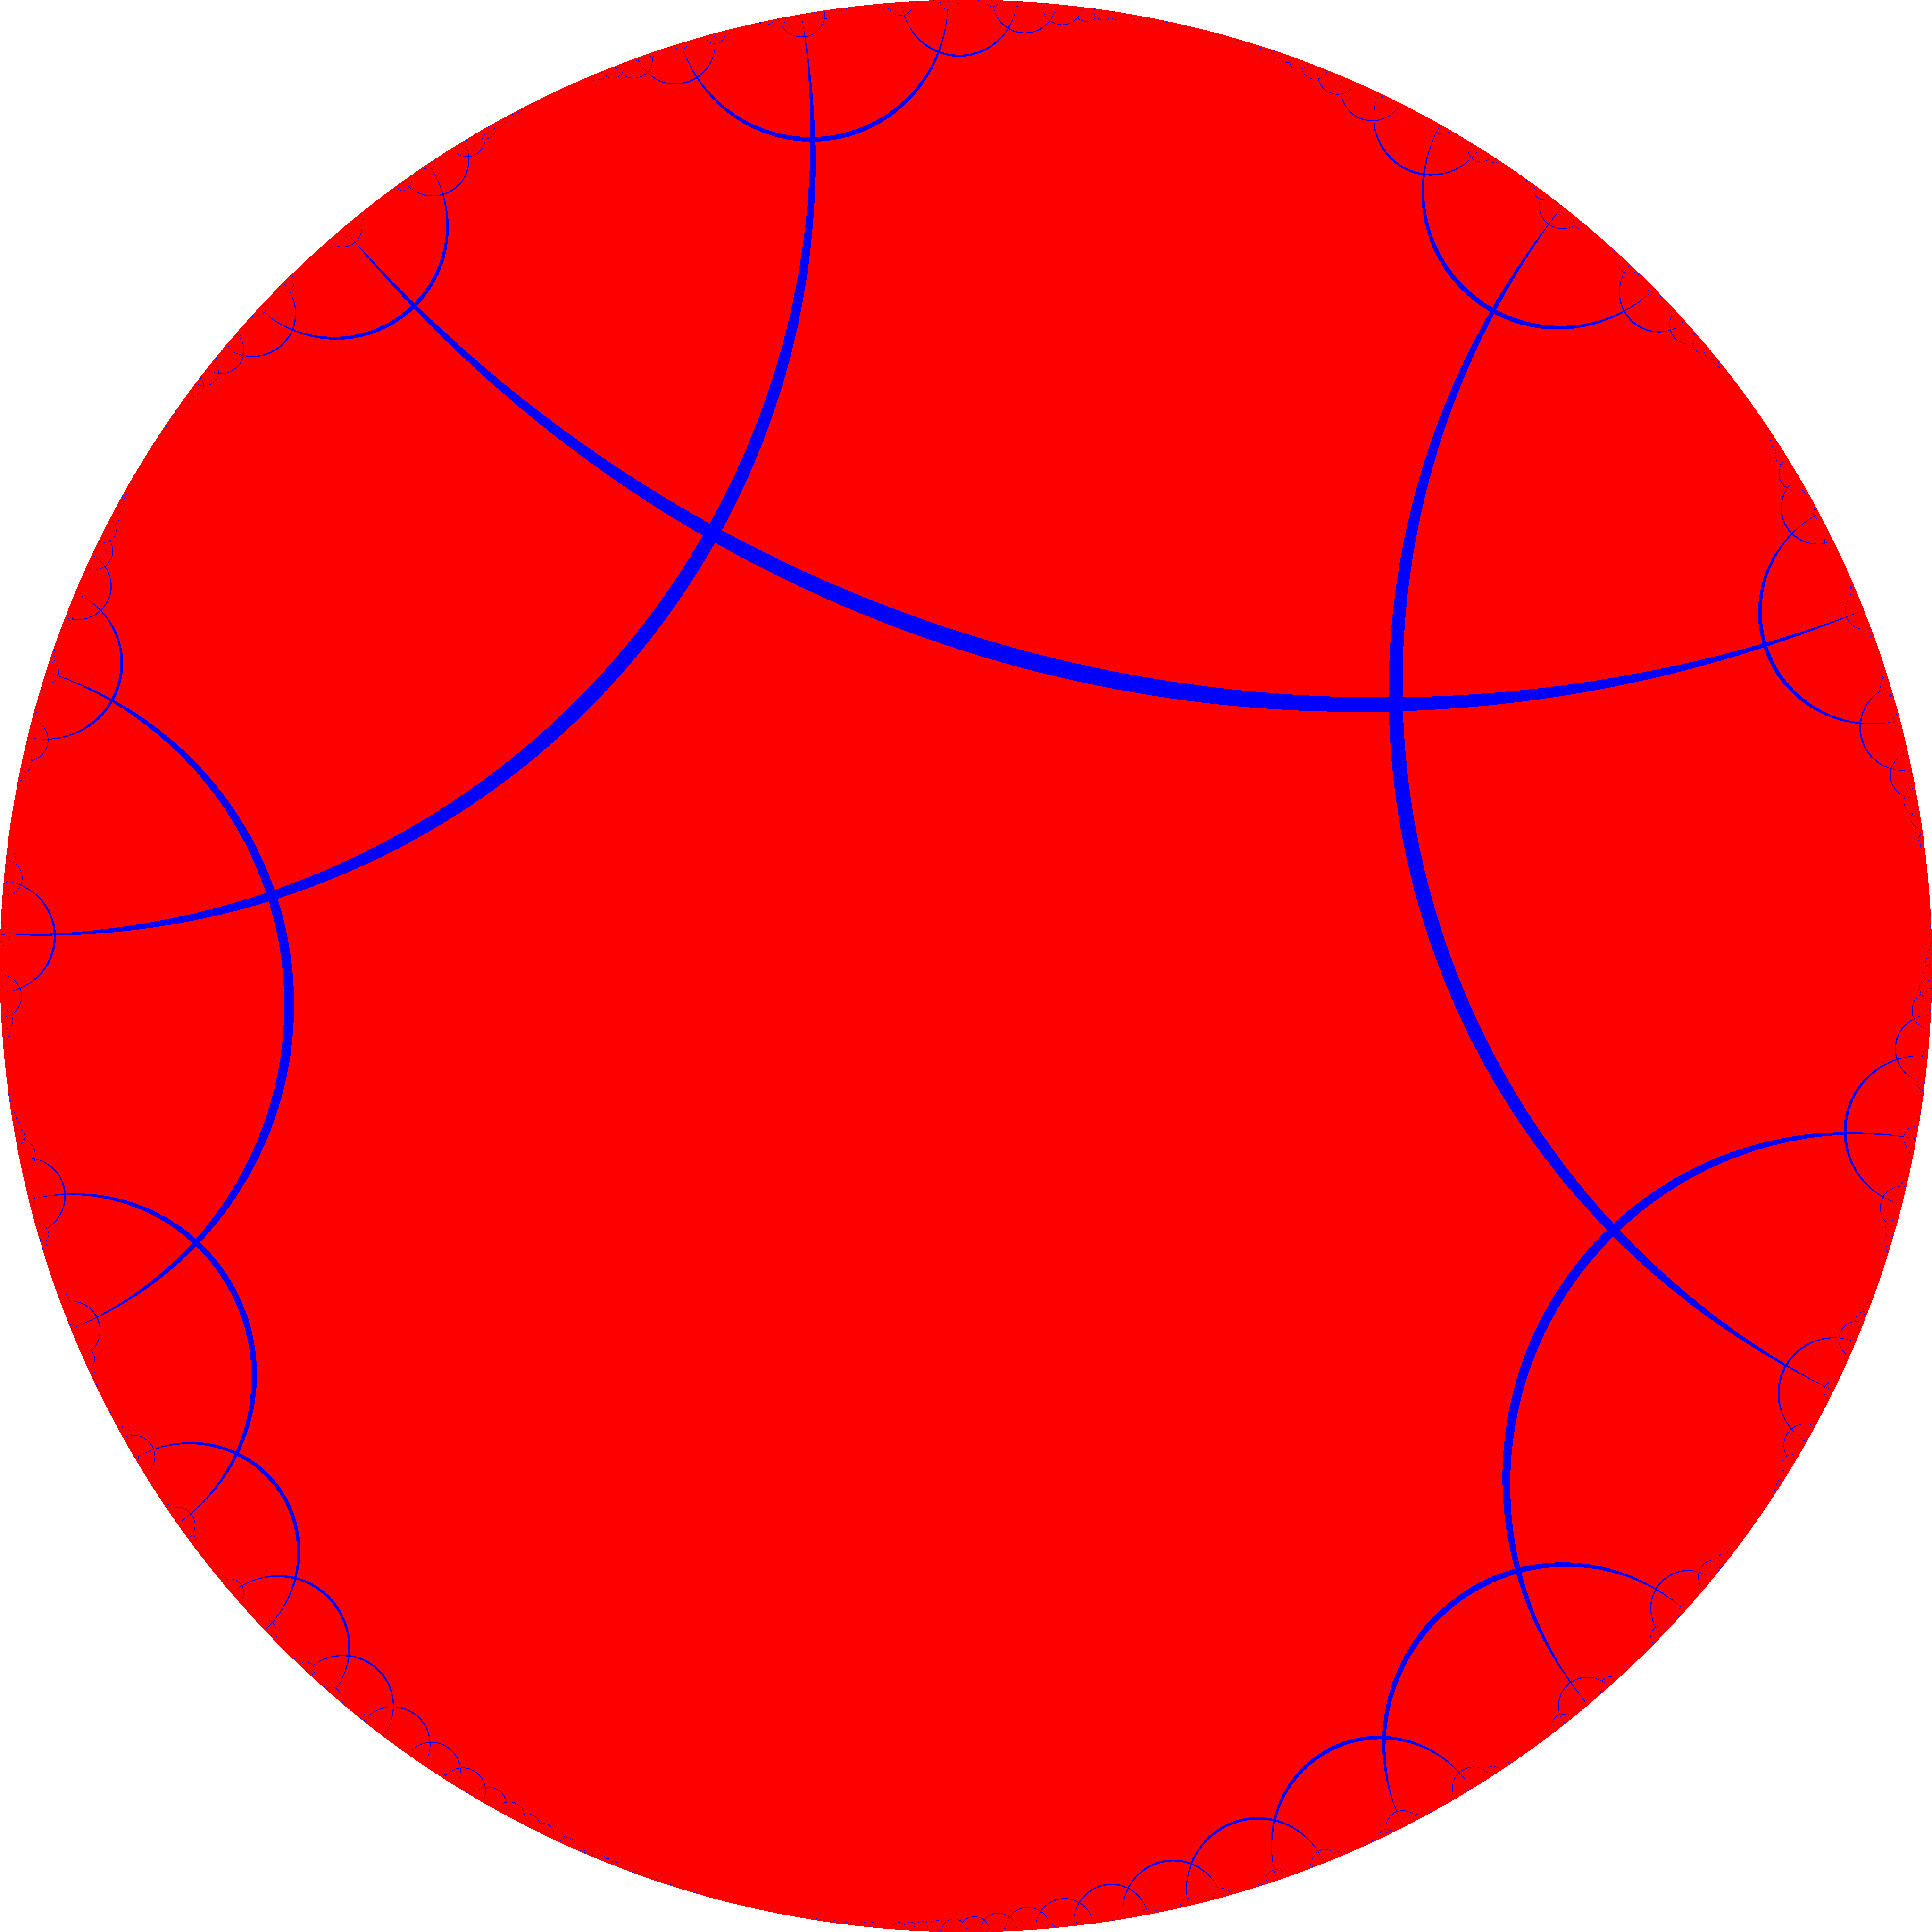
\includegraphics[width=6in]{images/t4096.png}};
    \draw (-4.40, +4.60) node[inner sep=1pt] (s) {$0 - 1$};
    \draw (-2.00, +2.80) node[inner sep=1pt] (z) {$0$};
    \draw (+2.90, +1.60) node[inner sep=1pt] (a) {$0 + 1$};
    \draw (+6.00, +1.60) node[inner sep=1pt] (aa) {$0 + 1 + 1$};
    \draw (+3.00, +5.00) node[inner sep=1pt] (am) {$(0 + 1) \cdot e$};
    \draw (+4.00, -2.00) node[inner sep=1pt] (ad) {$(0 + 1) / e$};
    \draw (-0.80, +6.20) node[inner sep=1pt] (m) {$0 \cdot e$};
    \draw (-4.90, +0.40) node[inner sep=1pt] (d) {$0 / e$};
\end{tikzpicture}
\caption{Embedding of the expressions}
\end{figure}

\section{A kind of new infinitesimal calculation}\label{sec:akonic}

\subsection{Local polar coordinate and flow equation}\label{sec:lpcafe}

Given any point $x_0$ on $\mathfrak{S}$, an additional axis $A$ pass $x_0$, then for any nearby point $x_1$, two
horocycle $B$ and $\bar{B}$ exists to connect with $x_0$ and $x_1$, so we can consider a local polar coordinate
$\mathfrak{C}_{x_0}$, in which $x_1$ decided by:
\begin{itemize}
    \item the angle $\theta$ between $A$ and $B$
    \item the length $\rho$ of arc between $x_0$ and $x_1$ along $B$
\end{itemize}

$\mathfrak{C}_{x_0}$ has a counterpart $\bar{\mathfrak{C}_{x_0}}$, in which $x_1$ decided by:
\begin{itemize}
    \item the angle $\bar{\theta}$ between $A$ and $\bar{B}$
    \item the length $\bar{\rho}$ of arc between $x_0$ and $x_1$ along $\bar{B}$
\end{itemize}

Question: what dose the two horocycles mean under the computation perspective? how dose the two horocycles contact?

Now we study infinitesimal calculation and horocycle flow on $\mathfrak{S}$. By the perspective of
addition-multiplication computation, under a local coordinate $\mathfrak{C}_{x_0}$,
consider a point moving from $x_0$ and towards $x_{\delta}$ with the angle $\theta$ and a small step $\epsilon$, we have

\begin{equation}
    x_{\delta} = (x_0 + \epsilon \cos \theta)(1 + \epsilon \sin \theta)
\end{equation}

or

\begin{equation}
    x_{\delta} = x_0 (1 + \epsilon \sin \theta) + \epsilon \cos \theta
\end{equation}

And both can be simplified to

\begin{equation}
    x_{\delta} = x_0 + \epsilon (x_0 \sin \theta + \cos \theta)
\end{equation}

So we have

\begin{equation}
    \frac{1}{\delta} (x_{\delta} - x_0) = \frac{\epsilon}{\delta} (\cos \theta + x_0 \sin \theta)
\end{equation}

We denote the left side of the above equation as $dx / dt$ when $\delta$ and $\epsilon$ approach 0.

\begin{equation}
    \frac{dx}{dt} = u (\cos \theta + x \sin \theta)
    \label{eqn:flow}
\end{equation}

where $u$ is the moving speed.

\subsection{background defined by flow equation}\label{sec:}

By assuming $u = 1$ and costant angle $\theta$, we have a background which can be descibed by a simpler formula,

\begin{equation}
    \frac{dx}{dt} = \cos \theta + x \sin \theta
\end{equation}

Then we have the solution:

\begin{equation}
   x = x_0 e^{t \sin \theta} + (e^{t \sin \theta} - 1) \cot \theta
\end{equation}

And then expand to

\begin{equation}
   x =  x_0 e^{t \sin \theta} + [1 + t \sin \theta + \frac{1}{2!} t\sin^2 \theta  + \frac{1}{3!} t \sin^3 \theta + ... - 1] \cot \theta
\end{equation}

Or

\begin{equation}
   x =  x_0 e^{t \sin \theta} + t \cos \theta + \frac{1}{2} \sin 2\theta (\frac{t^2}{2!} + \frac{t^3}{3!} \sin \theta + \frac{t^4}{4!} \sin^2 \theta + ...)
\end{equation}

\newpage

\subsection{Constant speed flow}\label{sec:csflow}

\subsubsection{$\sin t$}

\begin{equation}
    \frac{dx}{dt} = u (\cos \theta + x \sin \theta)
\end{equation}

\begin{equation}
    \frac{d(\sin t)}{dt} = u(\cos \theta + \sin t \sin \theta)
\end{equation}

\begin{equation}
    u(\cos \theta + \sin t \sin \theta) - \cos t = 0
\end{equation}

\begin{equation}
    u = \frac{\cos t}{\cos \theta + \sin t \sin \theta}
\end{equation}


\begin{figure}[ht]
\centering
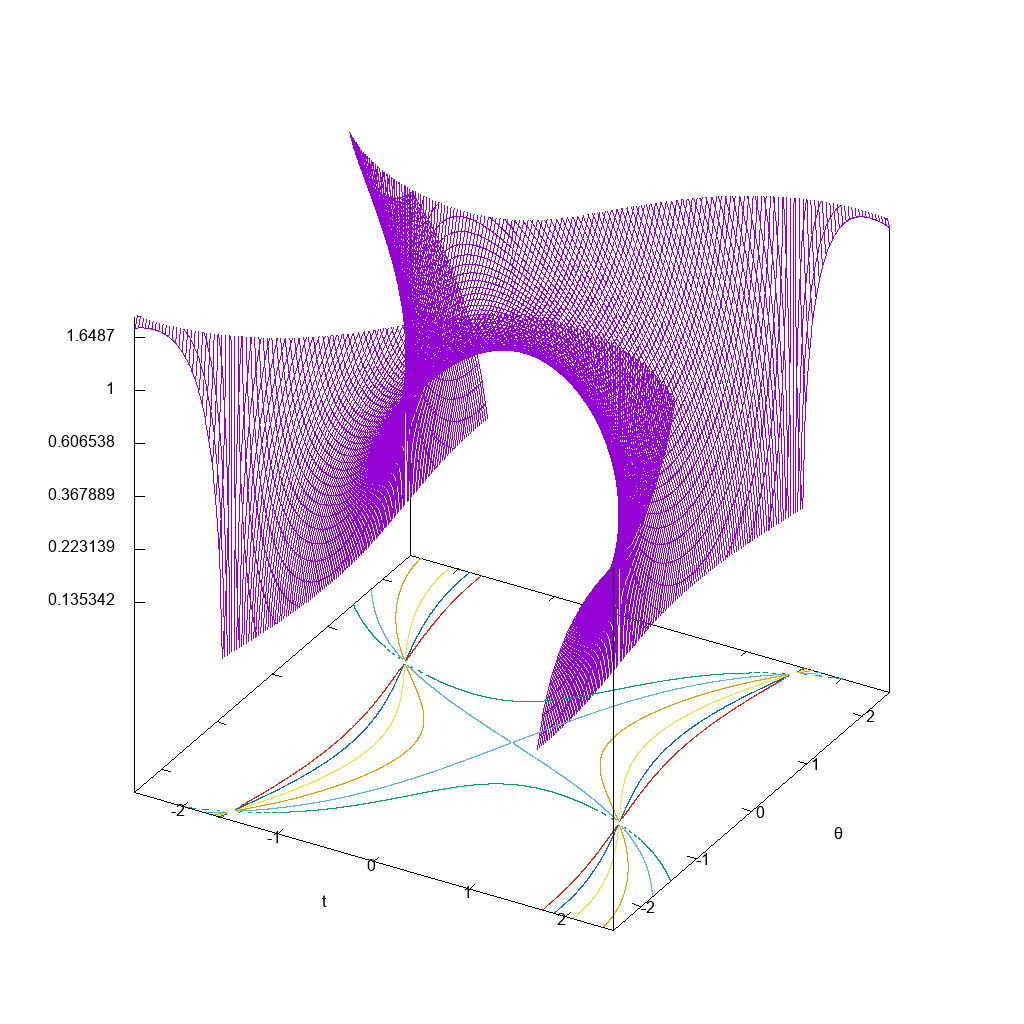
\includegraphics[width=5.5in]{plot/sine3d.png}
\caption{3d view of velocity $u(t, \theta)$ for process $\sin t$}
\end{figure}

\begin{figure}[ht]
\centering
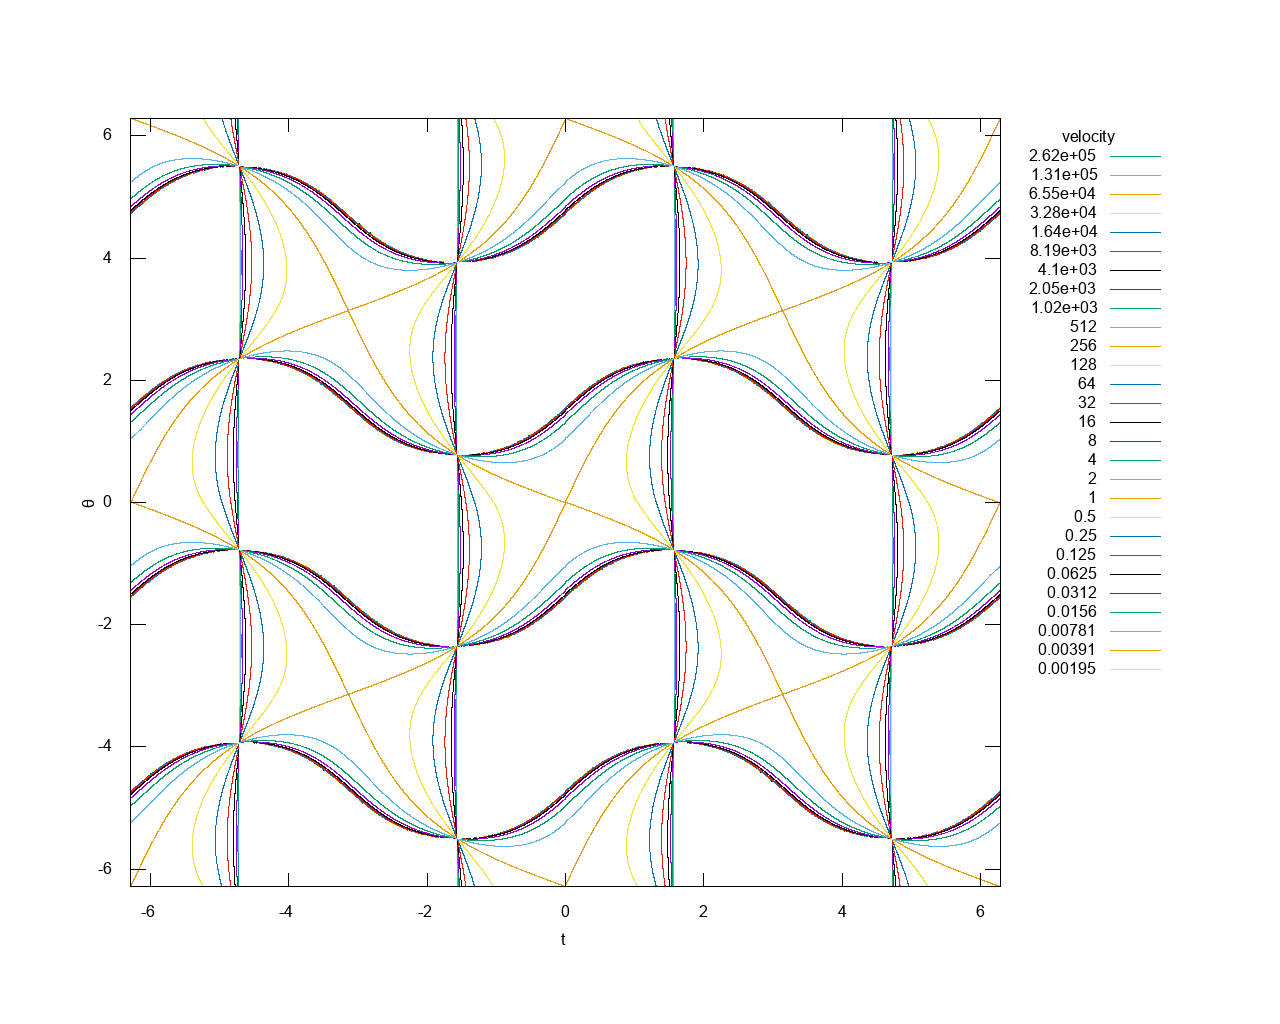
\includegraphics[width=5.5in]{plot/sine2d.png}
\caption{contour of velocity $u(t, \theta)$ for process $\sin t$}
\end{figure}

\subsection{Constant angle flow}

We guess constant angle flow is horocycle flow and there is a sign.

\subsubsection{Two examples of constant angle flow}

Assuming $\theta = \pi / 4$, we can conclude that

\begin{equation}
    \frac{dx}{dt} = \frac{\sqrt{2}}{2} (1 + x)
\end{equation}

\begin{equation}
    x = c e^{\frac{t}{\sqrt{2}}} - 1
\end{equation}

Then, we have below formula

\begin{equation}
    x = (x_0 + 1)e^{\frac{t}{\sqrt{2}}} - 1
\end{equation}

And a recurrence relation with $t_n = \sqrt{2} n$

\begin{equation}
    x_{n+1} = (x_n + 1) e - 1, n = 0 ... k ...
\end{equation}

or in simplified Polish notation

\begin{equation}
    x_{n+1} = [+*-] x_n, n = 0 ... k ...
\end{equation}

Geometricly, this recurrence relation defines a horecycle on $H^2$.

Assuming $\theta = \pi / 6$, we can conclude that

\begin{equation}
    \frac{dx}{dt} = \frac{1}{2} (\sqrt{3} x + 1)
\end{equation}

\begin{equation}
    x = c e^{\frac{\sqrt{3}}{2}t} - \frac{\sqrt{3}}{3}
\end{equation}

Then, we have below formula

\begin{equation}
    x = (x_0 + \frac{\sqrt{3}}{3})e^{\frac{\sqrt{3}}{2}t} - \frac{\sqrt{3}}{3}
\end{equation}

And a recurrence relation with $t_n = \frac{2\sqrt{3}}{3} n$

\begin{equation}
    x_{n+1} = (x_n + \frac{\sqrt{3}}{3}) e - \frac{\sqrt{3}}{3}, n = 0 ... k ...
\end{equation}

\subsubsection{Constant angle flow theorem}

\begin{theorem}
\label{l1}
A recurrence relation

\begin{equation}
    x_{n+1} = (x_n + \tan \theta) e - \tan \theta, n = 0 ... k ...
\end{equation}

is hold for a flow with constant angle $\theta$ and constant speed $\csc \theta$

\end{theorem}

\begin{proof}

We follow below solution of \eqref{eqn:flow}

\begin{equation}
   x = (\cot \theta + x_0) e^{t \sin \theta} - \cot \theta
\end{equation}

and re-write it as

\begin{equation}
   x = (\cot \theta + x_0) e^{t \sin \theta} - \cot \theta
\end{equation}

\end{proof}

\newpage

\section{The consistency problem}\label{sec:consistency}

The consistency of addition-multiplication tree, flow equation and hyperbolic geometrical structures

\subsection{A non-trival example of the consistency}

\subsection{How to formulate the consistency}

\subsection{A proof of the consistency}

\subsection{A new mathematical system $\mathfrak{S}$}

impact on learnability, predicability, efficency(time complexity, space complexity), energy cost

\newpage

\section{An embedding of surreal number}\label{sec:aeosn}

\section{A geometry of computation}\label{sec:gioc}

\newpage
\bibliographystyle{unsrt}
\bibliography{references}

\newpage
\appendix

\section{Derivation of the flow equation}

\begin{equation}
    \frac{dx}{dt} = \cos \theta + x \sin \theta
\end{equation}

We can get the solution by steps:

\begin{equation}
    \frac{dx}{\cos \theta + x \sin \theta} = dt
\end{equation}

\begin{equation}
    \frac{1}{\sin \theta} \frac{d(\cos \theta + x \sin \theta)}{\cos \theta + x \sin \theta} = dt
\end{equation}

\begin{equation}
    \frac{1}{\sin \theta} ln(\cos \theta + x \sin \theta) = t + C
\end{equation}

\begin{equation}
    \cos \theta + x \sin \theta = C e^{t \sin \theta}
\end{equation}

\begin{equation}
    \cos \theta + x_0 \sin \theta = C
\end{equation}

\begin{equation}
   x = \frac{\cos \theta + x_0 \sin \theta}{\sin \theta} e^{t \sin \theta} - \cot \theta
\end{equation}

\begin{equation}
   x = (\cot \theta + x_0) e^{t \sin \theta} - \cot \theta
\end{equation}

\begin{equation}
   x =  x_0 e^{t \sin \theta} + (e^{t \sin \theta} - 1) \cot \theta
\end{equation}

\begin{equation}
   x =  x_0 e^{t \sin \theta} + [1 + t \sin \theta + \frac{1}{2!} t\sin^2 \theta  + \frac{1}{3!} t \sin^3 \theta + ... - 1] \cot \theta
\end{equation}

\begin{equation}
   x =  x_0 e^{t \sin \theta} + t \cos \theta + \sin \theta \cos \theta (\frac{t^2}{2!} + \frac{t^3}{3!} \sin \theta + \frac{t^4}{4!} \sin^2 \theta + ...)
\end{equation}

\begin{equation}
   x =  x_0 e^{t \sin \theta} + t \cos \theta + \frac{1}{2} \sin 2\theta (\frac{t^2}{2!} + \frac{t^3}{3!} \sin \theta + \frac{t^4}{4!} \sin^2 \theta + ...)
\end{equation}

\begin{equation}
   x =  x_0 e^{t \sin \theta} + t \cos \theta + \frac{1}{2} \sin 2\theta (\frac{t^2}{2!} + \frac{t^3}{3!} \sin \theta + \frac{t^4}{4!} (\frac{1 - \cos 2\theta}{2}) + ...)
\end{equation}

When $\theta = \frac{k \pi}{2}, k = 0, 1, 2, 3...$, we have

\begin{equation}
    x = x_0 e^{t \sin \theta} + t \cos \theta
\end{equation}

rewrite it:

\begin{equation}
   x =  x_0 e^{t \sin \theta} + t \cos \theta + \frac{1}{2} \sin 2\theta \Psi(t)
\end{equation}

\begin{equation}
   \Psi(t) =  \frac{t^2}{2!} + \frac{t^3}{3!} \sin \theta + \frac{t^4}{4!} (\frac{1 - \cos 2\theta}{2}) + \frac{t^5}{5!} (\frac{3 \sin \theta - \sin 3\theta}{4}) + \frac{t^6}{6!} (\frac{3 - 4 \cos 2\theta - \cos 4\theta}{8}) + ...
\end{equation}

\begin{equation}
   \Psi(t) = c_0 + s_1 \sin \theta + c_2 \cos 2\theta + s_3 \sin 3\theta + c_4 \cos 4\theta + s_5 \sin 5\theta + c_6 \cos 6\theta + ...
\end{equation}

\begin{equation}
   c_0 = \frac{t^2}{2!} + \frac{1}{2}\frac{t^4}{4!} + \frac{3}{8} \frac{t^6}{6!} + \frac{5}{16} \frac{t^8}{8!} + \frac{35}{128} \frac{t^{10}}{10!}  ...
\end{equation}

\begin{equation}
   s_1 = \frac{t^3}{3!} + \frac{3}{4}\frac{t^5}{5!} + \frac{5}{8} \frac{t^7}{7!} + \frac{35}{64} \frac{t^9}{9!} + \frac{63}{128} \frac{t^{11}}{11!}  ...
\end{equation}

\begin{equation}
   c_2 = \frac{t^3}{3!} + \frac{3}{4}\frac{t^5}{5!} + \frac{5}{8} \frac{t^7}{7!} + \frac{35}{64} \frac{t^9}{9!} + \frac{63}{128} \frac{t^{11}}{11!}  ...
\end{equation}

\begin{equation}
   s_3 = \frac{t^3}{3!} + \frac{3}{4}\frac{t^5}{5!} + \frac{5}{8} \frac{t^7}{7!} + \frac{35}{64} \frac{t^9}{9!} + \frac{63}{128} \frac{t^{11}}{11!}  ...
\end{equation}

\begin{equation}
   c_4 = \frac{t^3}{3!} + \frac{3}{4}\frac{t^5}{5!} + \frac{5}{8} \frac{t^7}{7!} + \frac{35}{64} \frac{t^9}{9!} + \frac{63}{128} \frac{t^{11}}{11!}  ...
\end{equation}

\begin{equation}
   s_5 = \frac{t^3}{3!} + \frac{3}{4}\frac{t^5}{5!} + \frac{5}{8} \frac{t^7}{7!} + \frac{35}{64} \frac{t^9}{9!} + \frac{63}{128} \frac{t^{11}}{11!}  ...
\end{equation}

\begin{equation}
    {\left(C - \int \cos\left(\theta\left(t\right)\right) e^{\left(\int \sin\left(\theta\left(t\right)\right)\,{d t}\right)}\,{d t}\right)} e^{\left(-\int \sin\left(\theta\left(t\right)\right)\,{d t}\right)}
\end{equation}


\subsection{Other examples of driving charts}\label{sec:meodc}

\subsubsection{a constant k}

\begin{equation}
    0 = \cos \theta + k \sin \theta
\end{equation}

\begin{equation}
    \theta = n\pi - \arctan \frac{1}{k}
\end{equation}

\subsubsection{identity}

\begin{equation}
    \cos \theta + t \sin \theta - 1 = 0
\end{equation}

\begin{equation}
    \theta = 2k\pi
\end{equation}
\begin{equation}
    \theta = 2k\pi + \tan^{-1} t
\end{equation}

\subsubsection{inverse of t}

\begin{equation}
    \frac{d(t^{-1})}{dt} = \cos \theta + t^{-1} \sin \theta
\end{equation}

\begin{equation}
    t^2 \cos \theta + t \sin \theta + 1 = 0
\end{equation}

\subsubsection{square of t}

\begin{equation}
    \frac{d(t^2)}{dt} = \cos \theta + t^2 \sin \theta
\end{equation}

\begin{equation}
    \cos \theta + t^2 \sin \theta - 2 t = 0
\end{equation}

\subsubsection{cube of t}

\begin{equation}
    \frac{d(t^3)}{dt} = \cos \theta + t^3 \sin \theta
\end{equation}

\begin{equation}
    \cos \theta + t^3 \sin \theta - 3 t^2 = 0
\end{equation}

\subsubsection{sin of t}

\begin{equation}
    \frac{d(\sin t)}{dt} = \cos \theta + \sin t \sin \theta
\end{equation}

\begin{equation}
     \cos \theta + \sin t \sin \theta - \cos t = 0
\end{equation}

\subsubsection{exp of t}

\begin{equation}
    \frac{d(e^t)}{dt} = \cos \theta + e^t \sin \theta
\end{equation}

\begin{equation}
     \cos \theta + e^t \sin \theta - e^t = 0
\end{equation}

\end{document}
